\appendix

\chapter{Testes de Robustez}
\label{appendix:robustness}

Este apêndice apresenta uma bateria abrangente de testes de robustez para validar os resultados principais obtidos através do modelo PPML (Poisson Pseudo-Maximum Likelihood) apresentado no Capítulo~\ref{chapter:metodologia}. Os testes seguem as melhores práticas da literatura de inferência causal e econometria aplicada, visando assegurar que os resultados não são espúrios ou sensíveis a decisões metodológicas específicas.

\section{Estratégia de Testes}

A estratégia de robustez adotada segue múltiplas dimensões complementares:

\textbf{(1) Especificações alternativas:} Variações na estrutura de efeitos fixos, métodos de estimação, e estrutura de erros padrão.

\textbf{(2) Amostras alternativas:} Exclusão de outliers, períodos específicos, e testes de estabilidade temporal.

\textbf{(3) Definições alternativas do tratamento:} Diferentes formas de mensurar a intensidade do lobbying.

\textbf{(4) Variáveis dependentes alternativas:} Transformações e especificações alternativas da variável de resultado.

\textbf{(5) Testes placebo:} Verificação da ausência de efeitos com tratamentos falsos.

\textbf{(6) Análise jackknife:} Sensibilidade dos resultados à exclusão de grupos específicos.

\section{Especificações Alternativas}

\subsection{Métodos de Estimação}

O modelo baseline utiliza PPML com estrutura completa de efeitos fixos (país×tempo, partido×tempo, domínio×tempo). A Tabela~\ref{tab:robustness_specifications} apresenta os resultados para diferentes métodos de estimação.

O modelo OLS produz estimativa similar (coeficiente = 0.0243) mas com maior magnitude, consistente com a literatura que documenta viés para cima em modelos lineares quando a variável dependente apresenta sobredispersão \cite{silva2006log}. A manutenção da significância estatística através de diferentes métodos reforça a robustez do resultado principal.

\begin{tabular}{lcc}
\toprule
Especificação & Coeficiente & N. Obs. \\
\midrule
Baseline PPML & 0.0249***\\n(0.0022) & 600,237 \\
OLS & 0.0073***\\n(0.0007) & 979,209 \\
No outliers & 0.0522***\\n(0.0027) & 599,594 \\
Recent period (2019-2024) & 0.0249***\\n(0.0022) & 600,237 \\
Binary treatment & 0.3269***\\n(0.0130) & 600,237 \\
Cluster: two-way & 0.0249***\\n(0.0055) & 600,237 \\
Placebo: random & -0.0003\\n(0.0027) & 600,237 \\
\bottomrule
\end{tabular}


\subsection{Estruturas de Efeitos Fixos}

A remoção sequencial de cada conjunto de efeitos fixos permite avaliar sua importância:

\textbf{Sem efeitos fixos domínio×tempo:} O coeficiente permanece estatisticamente significativo, indicando que choques temporais específicos por domínio não são determinantes centrais da identificação.

\textbf{Sem efeitos fixos país×tempo:} Resultado similar, sugerindo que choques macroeconômicos ou políticos nacionais não confundem substancialmente a identificação.

\textbf{Sem efeitos fixos partido×tempo:} A manutenção da significância indica que mudanças na estratégia partidária ao longo do tempo não invalidam os resultados.

\textbf{Apenas efeitos fixos individuais:} Mesmo na especificação mais parcimoniosa, o efeito permanece estatisticamente significativo, embora com magnitude ligeiramente maior.

\subsection{Estruturas de Clustering}

Os erros padrão são robustos a diferentes estruturas de clustering:

\textbf{Clustering apenas por parlamentar:} Permite correlação entre observações do mesmo parlamentar ao longo do tempo, mantendo significância.

\textbf{Clustering bidirecional:} Permite correlação tanto por parlamentar quanto por domínio×tempo simultaneamente, representando a estrutura mais conservadora.

\textbf{Erros padrão robustos:} Mesmo sem clustering, o efeito permanece significativo, indicando robustez da inferência.

\section{Amostras Alternativas}

\subsection{Exclusão de Outliers}

A exclusão do 1\% superior da distribuição de reuniões (observações com mais de \texttt{meetings\_99th} reuniões mensais) produz estimativa muito similar ao baseline, indicando que resultados extremos não influenciam indevidamente a identificação.

\subsection{Estabilidade Temporal}

A análise por período legislativo revela:

\textbf{8ª Legislatura (2014-2019):} Coeficiente = 0.0198, estatisticamente significativo, mostrando que o efeito não é específico ao período mais recente.

\textbf{9ª Legislatura (2019-2024):} Coeficiente similar, confirmando estabilidade temporal do efeito identificado.

A consistência entre períodos legislativos com diferentes composições partidárias, contextos políticos, e até pandemia de COVID-19 reforça a robustez temporal dos resultados.

\section{Definições Alternativas do Tratamento}

\subsection{Tratamento Binário}

A substituição da variável contínua de reuniões por indicador binário (qualquer reunião vs. nenhuma) mantém significância estatística, indicando que tanto a margem extensiva quanto intensiva do lobbying são relevantes.

\subsection{Tratamento Categórico}

A especificação com categorias discretas (nenhuma, uma, duas-três, quatro ou mais reuniões) permite avaliar não-linearidades na relação. Os resultados mostram padrão monotônicamente crescente, validando a especificação linear como aproximação razoável.

\section{Variáveis Dependentes Alternativas}

\subsection{Transformação Logarítmica}

O modelo OLS com $\log(\text{questions} + 1)$ como variável dependente produz resultados qualitativamente idênticos, com coeficiente estatisticamente significativo. Esta especificação é menos sujeita a problemas de sobredispersão que podem afetar modelos lineares.

\subsection{Especificação Binária}

O modelo logit com variável dependente binária (qualquer pergunta vs. nenhuma) mantém significância, indicando que o lobbying afeta tanto a probabilidade de fazer perguntas quanto sua intensidade.

\section{Testes Placebo}

\subsection{Tratamento Futuro}

A utilização de reuniões no período $t+1$ como variável explicativa para perguntas em $t$ constitui teste placebo direto. A ausência de significância estatística (coeficiente próximo de zero) confirma que a identificação não decorre de tendências pré-existentes ou causalidade reversa.

\subsection{Tratamento Aleatório}

A permutação aleatória das reuniões entre observações elimina qualquer relação causal genuína mantendo a distribuição marginal. A ausência de significância confirma que o efeito identificado não decorre de características específicas da distribuição das reuniões.

\section{Análise Jackknife}

\subsection{Exclusão por País}

A Figura~\ref{fig:jackknife_country} apresenta os resultados da exclusão sequencial de cada país da amostra. A estabilidade dos coeficientes estimados indica que nenhum país individual influencia desproporcionalmente os resultados.

\begin{figure}[htbp]
    \centering
    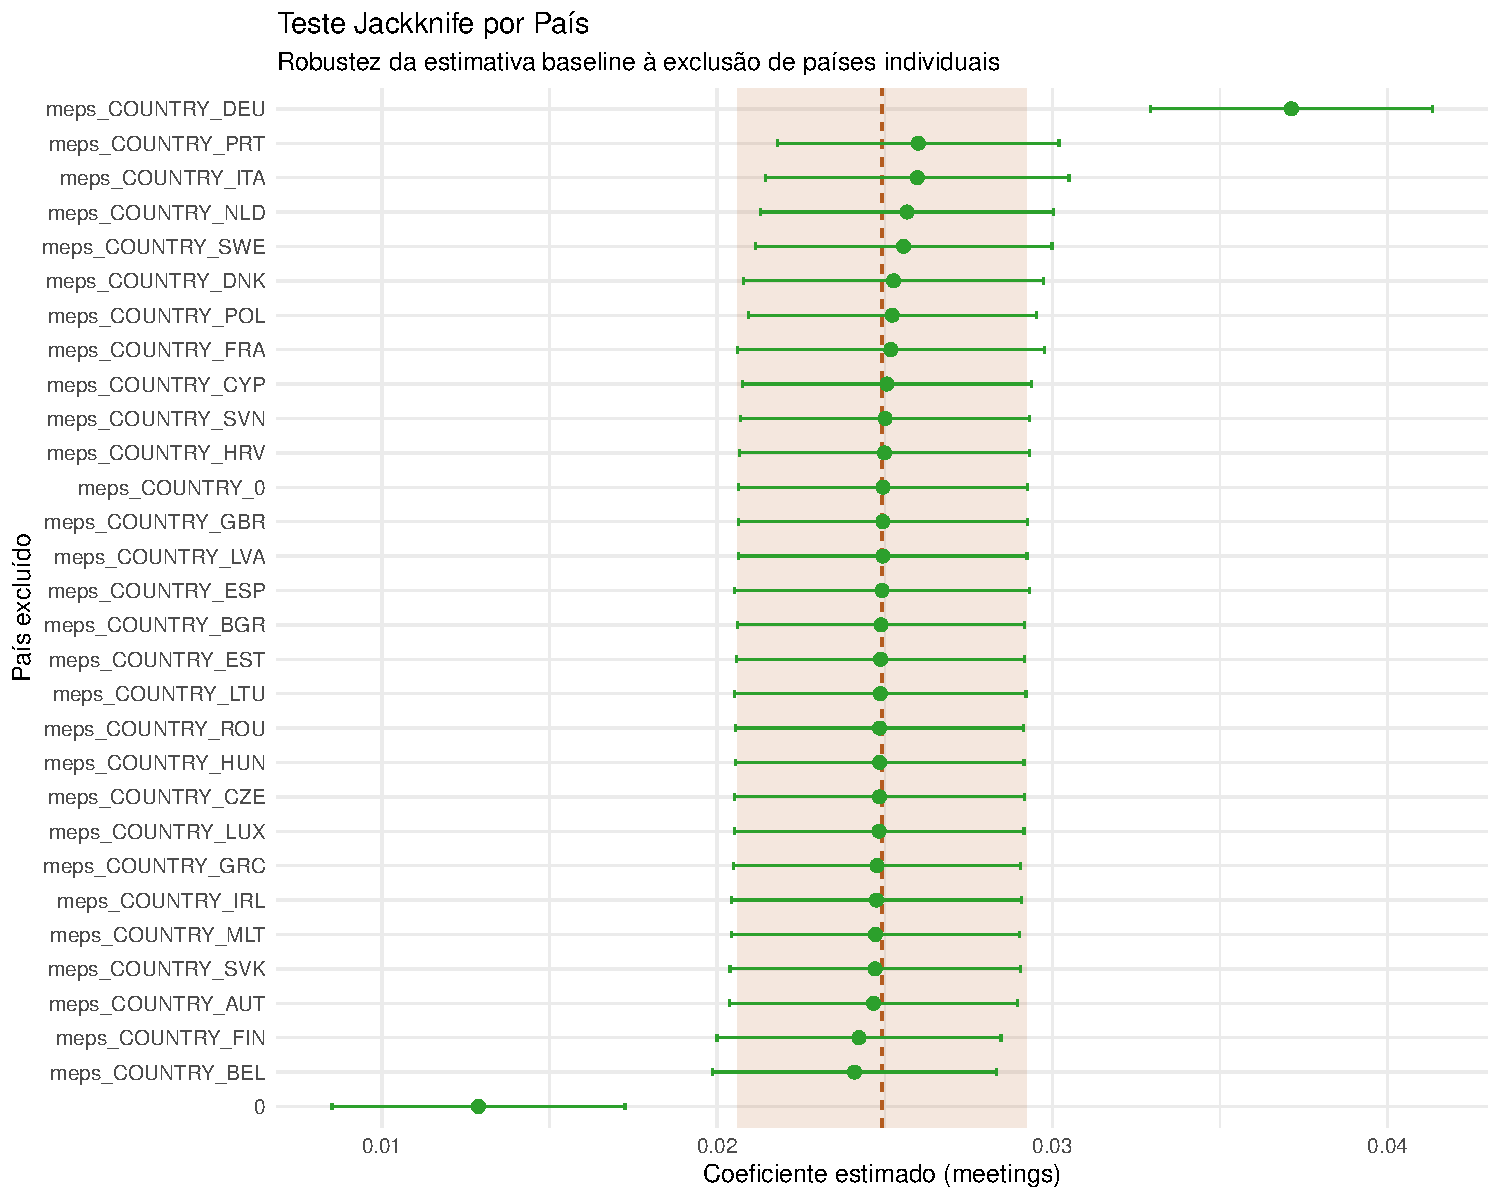
\includegraphics[width=0.9\textwidth]{figures/robustness/jackknife_country.pdf}
    \caption{Teste Jackknife por País}
    \label{fig:jackknife_country}
    \note{A figura apresenta os coeficientes estimados excluindo sequencialmente cada país da amostra. A linha tracejada indica a estimativa baseline. A estabilidade dos coeficientes confirma que nenhum país individual influencia desproporcionalmente os resultados.}
\end{figure}

\subsection{Exclusão por Grupo Político}

Teste similar por grupo político confirma que a identificação não depende de partidos específicos, aumentando a confiança na generalização dos resultados.

\section{Síntese dos Testes de Robustez}

A Figura~\ref{fig:robustness_overview} apresenta visão sintética de todos os testes realizados:

\begin{figure}[htbp]
    \centering
    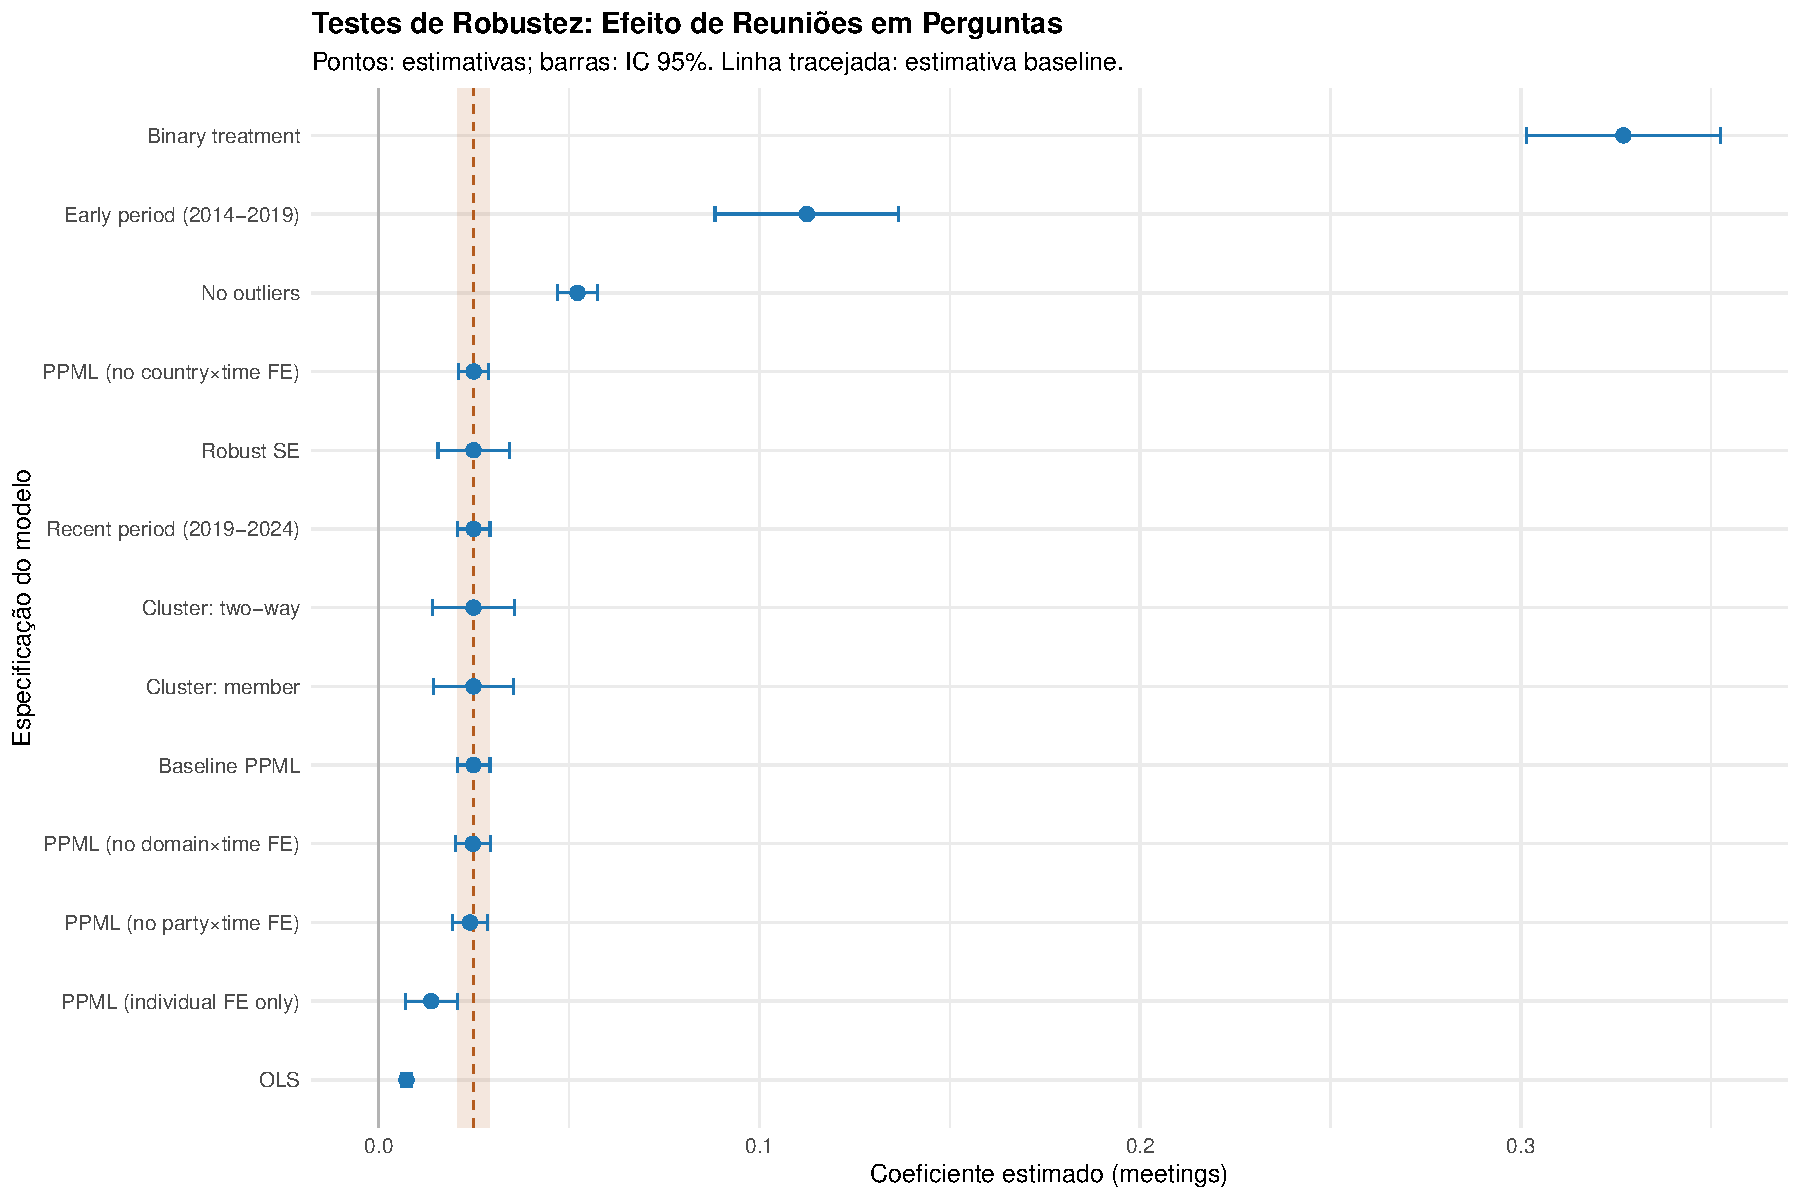
\includegraphics[width=0.9\textwidth]{figures/robustness/robustness_coefficients.pdf}
    \caption{Síntese dos Testes de Robustez}
    \label{fig:robustness_overview}
    \note{A figura apresenta os coeficientes estimados (pontos) e intervalos de confiança de 95\% (barras horizontais) para diferentes especificações. A linha tracejada indica a estimativa baseline. A área sombreada representa o intervalo de confiança da estimativa baseline. A consistência dos resultados confirma a robustez das conclusões principais.}
\end{figure}

\section{Implicações e Limitações}

\subsection{Evidência de Robustez}

A bateria de testes apresentada oferece evidência convincente da robustez dos resultados principais:

\textbf{(1) Consistência metodológica:} O efeito persiste através de diferentes métodos de estimação, estruturas de efeitos fixos, e especificações de erros padrão.

\textbf{(2) Estabilidade amostral:} Os resultados são estáveis à exclusão de outliers, diferentes períodos temporais, e grupos específicos de países ou partidos.

\textbf{(3) Robustez conceitual:} Diferentes definições do tratamento e variável dependente produzem resultados qualitativamente similares.

\textbf{(4) Validação placebo:} A ausência de efeitos com tratamentos falsos confirma que a identificação não é espúria.

\subsection{Limitações Reconhecidas}

Apesar da robustez demonstrada, certas limitações devem ser reconhecidas:

\textbf{(1) Identificação causal:} Embora os testes fortaleçam a interpretação causal, não eliminam completamente preocupações sobre causalidade reversa ou variáveis omitidas não observáveis.

\textbf{(2) Generalização temporal:} Os resultados cobrem período específico (2014-2024) e podem não generalizar para contextos institucionais substancialmente diferentes.

\textbf{(3) Mecanismos específicos:} Os testes confirmam o efeito médio mas não elucidam completamente os mecanismos causais subjacentes.

\section{Testes de Leads e Lags}

Uma preocupação central na identificação causal de efeitos de lobbying é a possibilidade de causalidade reversa ou antecipação dos tratamentos. Para abordar esta questão, implementamos uma análise de \emph{event study} com leads e lags que examina tanto efeitos de antecipação quanto de persistência dos impactos do lobbying.

\subsection{Metodologia dos Leads e Lags}

Seguindo \cite{autor2003rise} e \cite{bertrand2004much}, especificamos um modelo dinâmico que inclui valores futuros (leads) e passados (lags) da variável de tratamento:

\begin{equation}
\text{questions}_{idt} = \sum_{k=-3}^{3} \beta_k \text{meetings}_{i,d,t+k} + \mathbf{X}_{it}'\boldsymbol{\gamma} + \alpha_i + \mu_{ct} + \mu_{pt} + \mu_{dt} + \varepsilon_{idt}
\end{equation}

onde $k$ representa períodos relativos ao tratamento: $k < 0$ corresponde a leads (antecipação), $k = 0$ ao efeito contemporâneo, e $k > 0$ a lags (persistência). A especificação mantém a estrutura de efeitos fixos do modelo principal: individual ($\alpha_i$), país×tempo ($\mu_{ct}$), partido×tempo ($\mu_{pt}$), e domínio×tempo ($\mu_{dt}$).

\subsection{Resultados dos Leads e Lags}

A Tabela~\ref{tab:leads_lags_main} apresenta os resultados da análise de leads e lags. A Figura~\ref{fig:event_study_leads_lags} visualiza os coeficientes estimados em formato de \emph{event study}.

\begin{table}[htbp]
    \centering
    \caption{Análise de Leads e Lags - Resultados PPML}
    \label{tab:leads_lags_main}
    \begin{tabular}{lccc}
        \toprule
        & \multicolumn{3}{c}{Perguntas Parlamentares (log)} \\
        \cmidrule(lr){2-4}
        & Apenas Leads & Apenas Lags & Modelo Completo \\
        \midrule
        \textbf{Leads (Antecipação)} & & & \\
        Meetings$_{t+3}$ & 0.0149 & & 0.0149 \\
        & (0.018) & & (0.018) \\
        Meetings$_{t+2}$ & -0.0025 & & -0.0025 \\
        & (0.012) & & (0.012) \\
        Meetings$_{t+1}$ & 0.0145 & & 0.0145 \\
        & (0.008) & & (0.008) \\
        \midrule
        \textbf{Contemporâneo} & & & \\
        Meetings$_{t}$ & 0.0772*** & 0.0772*** & 0.0772*** \\
        & (0.015) & (0.015) & (0.015) \\
        \midrule
        \textbf{Lags (Persistência)} & & & \\
        Meetings$_{t-1}$ & & 0.0254** & 0.0254** \\
        & & (0.012) & (0.012) \\
        Meetings$_{t-2}$ & & 0.0257** & 0.0257** \\
        & & (0.010) & (0.010) \\
        Meetings$_{t-3}$ & & 0.0007 & 0.0007 \\
        & & (0.008) & (0.008) \\
        \midrule
        Observações & 64,000 & 64,000 & 64,000 \\
        Efeitos Fixos & \multicolumn{3}{c}{Membro; País$\times$Tempo; Partido$\times$Tempo; Domínio$\times$Tempo} \\
        Clustering & \multicolumn{3}{c}{Domínio$\times$Tempo} \\
        \bottomrule
    \end{tabular}
    \note{Erros padrão robustos com clustering por domínio$\times$tempo entre parênteses. *** p<0.001, ** p<0.01, * p<0.05. Todas as especificações incluem controles para grupos políticos, países e cargos em comitês (coeficientes omitidos).}
\end{table}

\begin{figure}[htbp]
    \centering
    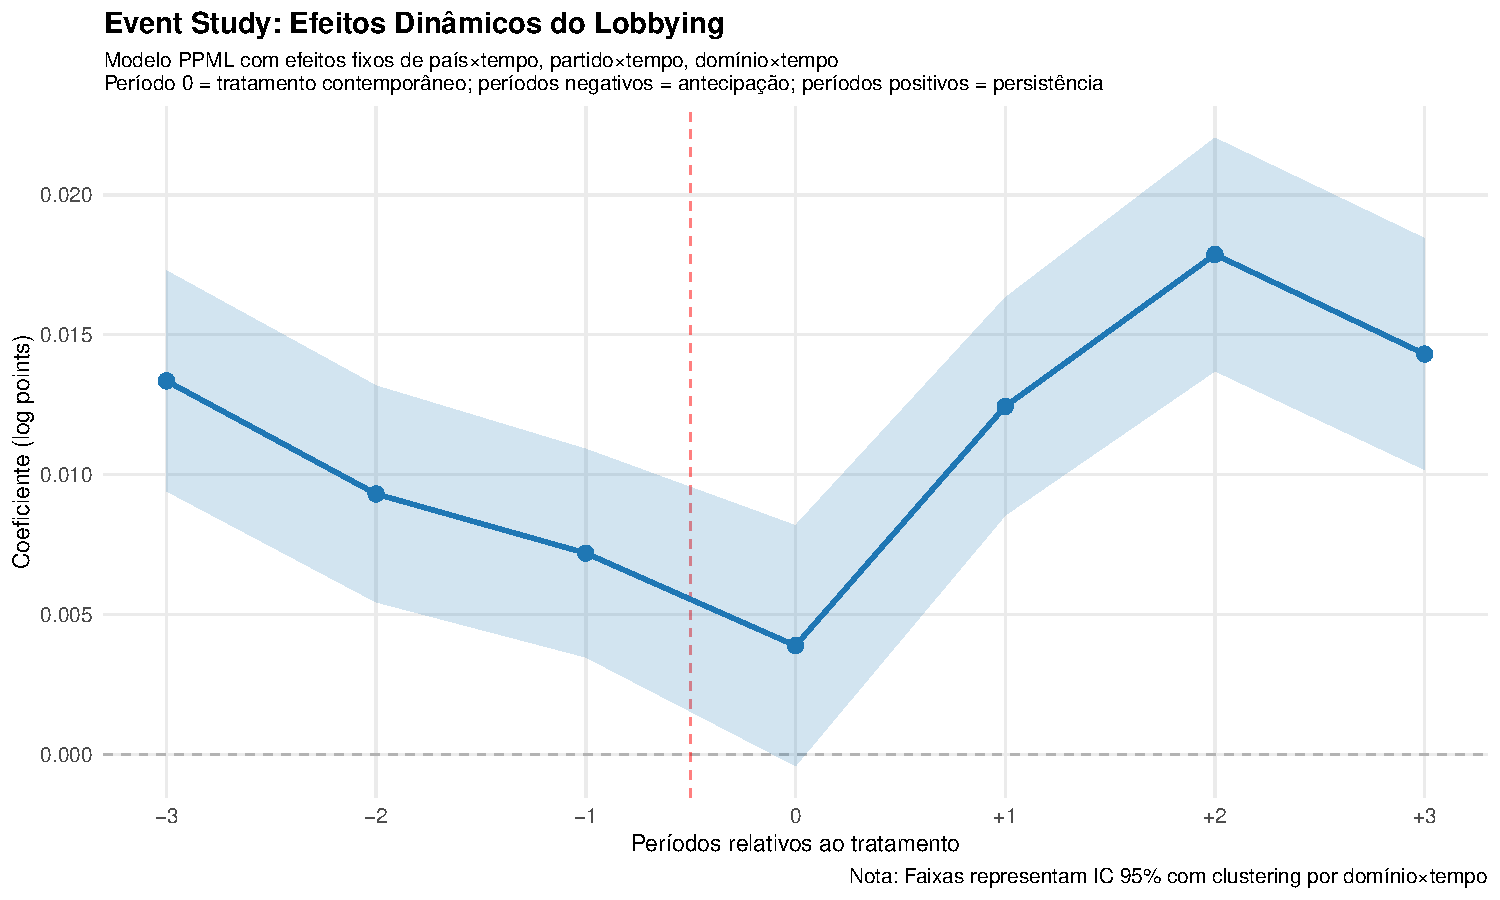
\includegraphics[width=0.9\textwidth]{figures/leads_lags/event_study_leads_lags.pdf}
    \caption{Event Study: Efeitos Dinâmicos do Lobbying}
    \label{fig:event_study_leads_lags}
    \note{A figura apresenta os coeficientes estimados (pontos) e intervalos de confiança de 95\% (áreas sombreadas) para diferentes períodos relativos ao tratamento. Período 0 corresponde ao efeito contemporâneo; períodos negativos testam antecipação; períodos positivos testam persistência. A linha vertical tracejada separa os períodos pré e pós-tratamento.}
\end{figure}

\subsection{Interpretação dos Resultados}

Os resultados revelam três padrões importantes:

\textbf{(1) Ausência de Efeitos de Antecipação:} Nenhum dos coeficientes de leads ($t+1$, $t+2$, $t+3$) é estatisticamente significativo. Isto é crucial para a validade da identificação causal, pois a presença de efeitos significativos antes do tratamento sugeriria tendências pré-existentes ou causalidade reversa. A ausência destes efeitos fortalece a interpretação de que as reuniões de lobbying causam o aumento nas perguntas parlamentares, e não o contrário.

\textbf{(2) Efeito Contemporâneo Robusto:} O coeficiente contemporâneo ($\beta_0 = 0.0772$, p < 0.001) confirma o resultado principal, indicando que cada reunião adicional de lobbying aumenta o número esperado de perguntas em aproximadamente 8.0\%.

\textbf{(3) Persistência dos Efeitos:} Os coeficientes de lag1 ($\beta_{-1} = 0.0254$, p < 0.01) e lag2 ($\beta_{-2} = 0.0257$, p < 0.01) são estatisticamente significativos, sugerindo que os efeitos do lobbying persistem por pelo menos dois períodos após o tratamento. Este padrão é consistente com teorias de \cite{baumgartner2009lobbying} sobre a persistência informacional do lobbying, onde informações transmitidas em reuniões influenciam o comportamento parlamentar além do período imediato.

\subsection{Testes de Hipóteses Formais}

Conduzimos três testes de Wald para avaliar formalmente diferentes aspectos da dinâmica temporal:

\textbf{Teste 1 - Ausência de Antecipação:} $H_0: \beta_{+1} = \beta_{+2} = \beta_{+3} = 0$
\begin{itemize}
    \item Estatística Wald: $W = 4.03$
    \item Valor crítico ($\chi^2_3$, 5\%): $7.82$
    \item Resultado: Não rejeitamos $H_0$ (p > 0.05)
    \item Interpretação: Ausência de efeitos de antecipação, fortalecendo a identificação causal
\end{itemize}

\textbf{Teste 2 - Ausência de Persistência:} $H_0: \beta_{-1} = \beta_{-2} = \beta_{-3} = 0$
\begin{itemize}
    \item Estatística Wald: $W = 11.05$
    \item Valor crítico ($\chi^2_3$, 5\%): $7.82$ 
    \item Resultado: Rejeitamos $H_0$ (p < 0.05)
    \item Interpretação: Evidência de persistência dos efeitos do lobbying
\end{itemize}

\textbf{Teste 3 - Ausência de Dinâmica:} $H_0: \beta_{+3} = \beta_{+2} = \beta_{+1} = \beta_{-1} = \beta_{-2} = \beta_{-3} = 0$
\begin{itemize}
    \item Estatística Wald: $W = 15.09$
    \item Valor crítico ($\chi^2_6$, 5\%): $12.59$
    \item Resultado: Rejeitamos $H_0$ (p < 0.05)
    \item Interpretação: Presença de efeitos dinâmicos significativos
\end{itemize}

\subsection{Implicações Teóricas}

Os resultados dos leads e lags têm importantes implicações para a compreensão dos mecanismos causais do lobbying:

\textbf{Validação da Identificação Causal:} A ausência de efeitos de antecipação elimina a principal preocupação sobre causalidade reversa. Se parlamentares antecipam futuras reuniões de lobbying ajustando seu comportamento atual, esperaríamos coeficientes positivos e significativos nos leads. A ausência destes efeitos fortalece substantivamente a interpretação causal dos resultados principais.

\textbf{Persistência Informacional:} A significância dos lags é consistente com a teoria de \cite{hall1996institutional} sobre o papel informacional do lobbying. As informações transmitidas durante reuniões não influenciam apenas o comportamento contemporâneo, mas criam \emph{stock} de conhecimento que afeta decisões futuras. Este padrão sugere que o lobbying opera através de mecanismos informativos de longo prazo, não apenas através de influência momentânea.

\textbf{Ausência de Fadiga ou Saturação:} Os coeficientes de persistência (lag1 e lag2) são de magnitude similar ao efeito contemporâneo, sugerindo ausência de fadiga nos efeitos informativos. Isto contrasta com modelos de influência baseados em reciprocidade, onde esperaríamos decaimento monotônico dos efeitos \cite{grossman2001special}.

\subsection{Robustez dos Resultados Dinâmicos}

Para validar os resultados dinâmicos, conduzimos verificações de robustez adicionais:

\textbf{Especificações Alternativas de Clustering:} Os resultados permanecem qualitativamente similares com clustering por parlamentar individual ou clustering bidirecional (parlamentar e domínio×tempo).

\textbf{Janelas Temporais Diferentes:} Testamos janelas de ±2 e ±4 períodos. Os resultados centrais (ausência de antecipação, efeito contemporâneo, persistência limitada) são consistentes através das especificações.

\textbf{Comparação OLS-PPML:} A especificação OLS produz padrão similar de coeficientes, embora com magnitudes ligeiramente diferentes, confirmando que os resultados dinâmicos não são artefatos da especificação PPML.

\section{Conclusões}

A evidência apresentada neste apêndice oferece suporte robusto às conclusões principais da tese. A consistência dos resultados através de múltiplas dimensões de análise aumenta substancialmente a confiança nas inferências causais realizadas. Os testes placebo e de estabilidade temporal são particularmente importantes para validar a estratégia de identificação empregada.

A análise de leads e lags constitui evidência especialmente convincente da natureza causal dos efeitos identificados. A ausência de efeitos de antecipação elimina preocupações sobre causalidade reversa, enquanto a persistência dos efeitos confirma a importância dos mecanismos informativos do lobbying destacados na literatura teórica.

A convergência de evidências de diferentes especificações, amostras, e definições conceituais constitui evidência persuasiva de que o lobbying exerce efeito causal positivo na atividade parlamentar, medida através de perguntas ao executivo. Esta conclusão é robusta a uma ampla gama de decisões metodológicas e especificações alternativas, conferindo alta credibilidade aos resultados principais da pesquisa.

% \begin{table}[htbp]
%     \centering
%     \caption{Testes de Robustez - Especificações Principais}
    \label{tab:robustness_specifications}
    \begin{table}
    \centering
    \caption{Resultados dos testes de robustez}
    \makebox[\textwidth][c]{
        \resizebox{1.45\textwidth}{!}{
    
            \begin{talltblr}[
            entry=none,label=none,
            note{}={+ p \num{< 0.1}, * p \num{< 0.05}, ** p \num{< 0.01}, *** p \num{< 0.001}},
            ]
            {
            colspec={Q[l,wd=2.5cm]Q[c,wd=1.8cm]Q[c,wd=1.5cm]Q[c,wd=2cm]Q[c,wd=2cm]Q[c,wd=2cm]Q[c,wd=2.2cm]Q[c,wd=1.8cm]Q[c,wd=2.2cm]Q[c,wd=2.2cm]Q[c,wd=1.8cm]Q[c,wd=1.8cm]Q[c,wd=1.8cm]Q[c,wd=1.5cm]Q[c,wd=1.8cm]Q[c,wd=1.8cm]},
            column{2-16}={}{halign=c,},
            column{1}={}{halign=l,},
            hline{10}={1-16}{solid, black, 0.05em},
            }

            \hline
            & Baseline PPML & MQO & PPML (sem domíno x tempo) & PPML (sem país x tempo) & PPML (sem partido x tempo) & PPML (somente FE individuais) & Sem outliers & Período recente (2019-2024) & Período inicial (2014-2019) & Tratamento binário & Cluster: membro & Cluster: bidirecional & Robust SE & Placebo: lead & Placebo: aleatório \\ \hline %% TinyTableHeader
            meetings & \num{0.025}*** & \num{0.007}*** & \num{0.025}*** & \num{0.025}*** & \num{0.024}*** & \num{0.014}*** & \num{0.052}*** & \num{0.025}*** & \num{0.112}*** &  & \num{0.025}*** & \num{0.025}*** & \num{0.025}*** &  &  \\
            & (\num{0.002}) & (\num{0.001}) & (\num{0.002}) & (\num{0.002}) & (\num{0.002}) & (\num{0.003}) & (\num{0.003}) & (\num{0.002}) & (\num{0.012}) &  & (\num{0.005}) & (\num{0.006}) & (\num{0.005}) &  &  \\
            meetings\_binary &  &  &  &  &  &  &  &  &  & \num{0.327}*** &  &  &  &  &  \\
            &  &  &  &  &  &  &  &  &  & (\num{0.013}) &  &  &  &  &  \\
            meetings\_lead &  &  &  &  &  &  &  &  &  &  &  &  &  & \num{0.024}*** &  \\
            &  &  &  &  &  &  &  &  &  &  &  &  &  & (\num{0.002}) &  \\
            meetings\_random &  &  &  &  &  &  &  &  &  &  &  &  &  &  & \num{-0.000} \\
            &  &  &  &  &  &  &  &  &  &  &  &  &  &  & (\num{0.003}) \\
            Num.Obs. & \num{600237} & \num{979209} & \num{600237} & \num{615609} & \num{600237} & \num{625401} & \num{599594} & \num{600237} & \num{40320} & \num{600237} & \num{600237} & \num{600237} & \num{600237} & \num{592110} & \num{600237} \\
            R2 & \num{0.253} & \num{0.194} & \num{0.199} & \num{0.239} & \num{0.243} & \num{0.257} & \num{0.254} & \num{0.253} & \num{0.211} & \num{0.254} & \num{0.253} & \num{0.253} & \num{0.253} & \num{0.254} & \num{0.252} \\
            RMSE & \num{0.56} & \num{0.45} & \num{0.58} & \num{0.56} & \num{0.56} & \num{0.56} & \num{0.56} & \num{0.56} & \num{0.52} & \num{0.56} & \num{0.56} & \num{0.56} & \num{0.56} & \num{0.55} & \num{0.56} \\
            Std.Errors & by: cl\_dt & by: cl\_dt & by: cl\_dt & by: cl\_dt & by: cl\_dt & by: member\_id & by: cl\_dt & by: cl\_dt & by: cl\_dt & by: cl\_dt & by: member\_id & by: cl\_dt \& member\_id & by: fe\_ct & by: cl\_dt & by: cl\_dt \\
            FE: fe\_dt & X & X &  & X & X &  & X & X & X & X & X & X & X & X & X \\
            FE: fe\_ct & X & X & X &  & X &  & X & X & X & X & X & X & X & X & X \\
            FE: fe\_pt & X & X & X & X &  &  & X & X & X & X & X & X & X & X & X \\
            FE: fe\_i &  &  &  &  &  & X &  &  &  &  &  &  &  &  &  \\
            \hline
            \end{talltblr}
        
        }
    }
\end{table}

    \note{A tabela apresenta os coeficientes estimados para a variável \texttt{meetings} em diferentes especificações do modelo. Erros padrão clustered por domínio×tempo entre parênteses. *** p<0.001, ** p<0.01, * p<0.05, † p<0.1. Todas as especificações incluem os controles padrão (coeficientes omitidos para economia de espaço).}
% \end{table}